\documentclass[conference]{IEEEtran}



% *** GRAPHICS RELATED PACKAGES ***
%
\ifCLASSINFOpdf
  % \usepackage[pdftex]{graphicx}
  % declare the path(s) where your graphic files are
  % \graphicspath{{../pdf/}{../jpeg/}}
  % and their extensions so you won't have to specify these with
  % every instance of \includegraphics
  % \DeclareGraphicsExtensions{.pdf,.jpeg,.png}
\else
  % or other class option (dvipsone, dvipdf, if not using dvips). graphicx
  % will default to the driver specified in the system graphics.cfg if no
  % driver is specified.
  % \usepackage[dvips]{graphicx}
  % declare the path(s) where your graphic files are
  % \graphicspath{{../eps/}}
  % and their extensions so you won't have to specify these with
  % every instance of \includegraphics
  % \DeclareGraphicsExtensions{.eps}
\fi
% graphicx was written by David Carlisle and Sebastian Rahtz. It is
% required if you want graphics, photos, etc. graphicx.sty is already
% installed on most LaTeX systems. The latest version and documentation
% can be obtained at: 
% http://www.ctan.org/pkg/graphicx
% Another good source of documentation is "Using Imported Graphics in
% LaTeX2e" by Keith Reckdahl which can be found at:
% http://www.ctan.org/pkg/epslatex
%
% latex, and pdflatex in dvi mode, support graphics in encapsulated
% postscript (.eps) format. pdflatex in pdf mode supports graphics
% in .pdf, .jpeg, .png and .mps (metapost) formats. Users should ensure
% that all non-photo figures use a vector format (.eps, .pdf, .mps) and
% not a bitmapped formats (.jpeg, .png). The IEEE frowns on bitmapped formats
% which can result in "jaggedy"/blurry rendering of lines and letters as
% well as large increases in file sizes.
%
% You can find documentation about the pdfTeX application at:
% http://www.tug.org/applications/pdftex





\usepackage{amsmath}


\usepackage[utf8]{inputenc}
\usepackage{url}
\usepackage{hyperref}
\usepackage{graphicx}


% acckorrect bad hyphenation here
\hyphenation{op-tical net-works semi-conduc-tor}


\begin{document}
\title{}


% author names and affiliations
% use a multiple column layout for up to three different
% affiliations
\author{}


% make the title area
\maketitle

% As a general rule, do not put math, special symbols or citations
% in the abstract
\begin{abstract}
\end{abstract}

\section{Introduction}


\section{Related work}


\section{Solution}

To solve these issues, we propose a modular architecture from which will stem a unified platform in which the benchmarks can be run. The main benefits of such a platform are twofold: to provide a common ground in which the middlewares can be benchmarked to ensure equal an playing field, and to ease the addition of other subsequent middlewares. This is achieved by factoring the common elements that go in the creation of any benchmarking application. The main building blocks of our architecture are visible in figure~\ref{fig:main_building_blocks}.

\begin{figure}[htbp!]
  \centering
  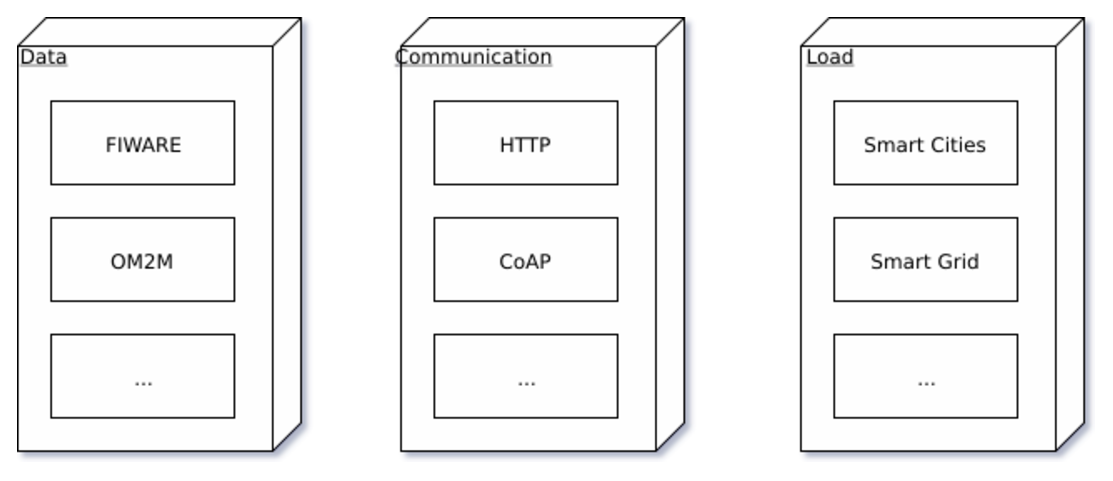
\includegraphics[width=\linewidth]{figures/benchmark_blocks.eps}
  \caption{Main architecture building blocks}
  \label{fig:main_building_blocks}
\end{figure}

The goal is to only implement what is necessary for a new entry in the benchmarking platform instead of using a similar implementation for each one. We propose a communication block where the communication protocols are lodged, such as HTTP or CoAP, and each has the methods implemented, such as POST or GET, so that they are totally platform independent and can be reused. If a new protocol is required to be added to the platform, its methods can be implemented without interfering with the remaining structure.

The data block is where the middleware specific functions reside, and each of these is responsible for implementing its data structure and bridging the gap to the protocols. Similarly to the data block, it is designed so that each is independent so that all can use the same communication methods implemented in the communication block. With a new entry, one can observe how the existing ones are structured, thereby speeding up the process and keeping it isolated without interfering with the existing setup. 

The load block will enable different types of IoT scenarios to be programmed and dynamically changed, so that we can attempt to mimic real world scenarios such as Smart Cities. Again, this should be independent from each of the other blocks so that the same workloads can be used throughout all middlewares and protocols, providing a basis for comparison and ensuring high flexibility.

Each building block will have several sub-blocks, which will correspond to a given class. In an initial phase, we attempted to create an application to benchmark the OM2M with a basis on the work conducted in~\cite{pereira_benchmarking_2018} and \cite{cardoso_benchmarking_2017} , while keeping it as generic as possible to enable future middleware additions and follow our architecture guidelines. This resulted in the structure visible in

\begin{figure}[htbp!]
  \centering
  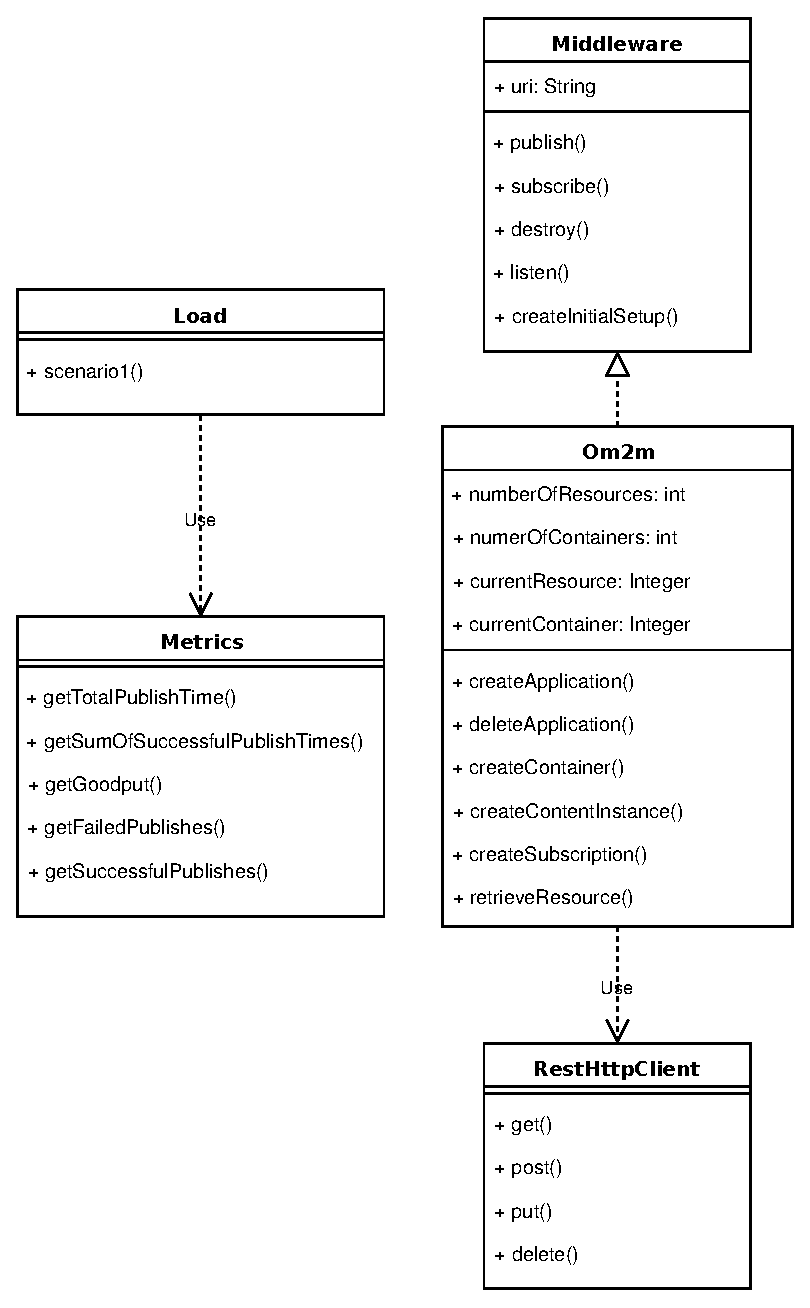
\includegraphics[width=\linewidth]{figures/class_diagram.eps}
  \caption{Class diagram for the initial platform stage}
  \label{fig:class_diagram_om2m}
\end{figure}

\section{Evaluation}


\section{Conclusion}



% trigger a \newpage just before the given reference
% number - used to balance the columns on the last page
% adjust value as needed - may need to be readjusted if
% the document is modified later
%\IEEEtriggeratref{8}
% The "triggered" command can be changed if desired:
%\IEEEtriggercmd{\enlargethispage{-5in}}

% references section

% can use a bibliography generated by BibTeX as a .bbl file
% BibTeX documentation can be easily obtained at:
% http://mirror.ctan.org/biblio/bibtex/contrib/doc/
% The IEEEtran BibTeX style support page is at:
% http://www.michaelshell.org/tex/ieeetran/bibtex/
%\bibliographystyle{IEEEtran}
% argument is your BibTeX string definitions and bibliography database(s)
%\bibliography{IEEEabrv,../bib/paper}
%
% <OR> manually copy in the resultant .bbl file
% set second argument of \begin to the number of references
% (used to reserve space for the reference number labels box)

\bibliographystyle{unsrt}
\bibliography{biblio}


% that's all folks
\end{document}


%%% Local Variables:
%%% mode: latex
%%% TeX-master: t
%%% End:
=======
\documentclass{article}
\usepackage[utf8]{inputenc}
\begin{document}
(Type your content here.)
\end{document}
>>>>>>> f2e640db19cf7ec24c539f6c2c2fad5a3c77c44d
